\documentclass[12pt,a4paper]{ctexart}

\usepackage{../../Styles/mystyle-report}

\graphicspath{{./image/}}% 指定图片目录，后续可以直接使用图片文件名。

% 去掉交叉引用方框
\hypersetup{
colorlinks=true,    % 启用彩色链接（替代方框）
linkcolor=black,    % 图表/章节引用 纯黑色（无框）
citecolor=black,    % 文献引用 纯黑色
urlcolor=blue       % 网址保留蓝色
}

% 重定义section左对齐
\makeatletter
% 重定义 \section 命令（一级标题）
\renewcommand{\section}{\@startsection{section}{1}{\z@}%
% 参数4：标题 上方 的空白距离（负数是固定写法）
{-0ex \@plus -1ex \@minus -.2ex}%
% 参数5：标题 下方 的空白距离（标题和正文之间的距离）
{2.3ex \@plus.2ex}%
% 参数6：标题样式：默认字体+大号+加粗+左对齐
{\normalfont\Large\bfseries\raggedright}}
% 关闭内部命令权限（成对使用）加\raggedright实现左对齐
\makeatother

\pagestyle{fancy}
\fancyhf{} % 清空默认页眉页脚

% 页眉：右侧章节，左侧页码（右侧页码去掉了)
% \fancyhead[L]{\zihao{5} \thepage}
\fancyhead[R]{\zihao{5} \leftmark}

% 页码放到 页面底部 正中间
\fancyfoot[C]{\zihao{5} \thepage}

% 页眉细横线
\renewcommand{\headrulewidth}{0.5pt}

% 让\section自动生成页眉标记
\renewcommand{\sectionmark}[1]{\markboth{\thesection\quad #1}{}}

% 标题页样式：无页眉、无页码
\fancypagestyle{titlepage}{
\fancyhf{}
\renewcommand{\headrulewidth}{0pt}
\renewcommand{\footrulewidth}{0pt}
}

% 标题、作者信息
% \title{\heiti 25-26-2学期时间序列分析实训课程实验报告}
% \date{\today}
% \author{\textbf{姓名：\underline{\quad 邹文杰 \quad} \quad 序号：\underline{\quad 80 \quad}}}

\begin{document}

\thispagestyle{empty}  % 去掉了第一页页码

\vspace*{\fill}  % 顶部自动填充空白（垂直居中）
\begin{center}
\heiti \Huge 25-26-2 学期时间序列分析实训课程实验报告(二) \\[1.8cm]

% 日期放在上方
\Large \today \\[1.2cm]

% 姓名+序号放在下方
\Large 姓名：\underline{\quad 邹文杰 \quad} \quad\quad 序号：\underline{\quad 80 \quad}
\end{center}
\vfill  % 底部自动填充空白（垂直居中）

\newpage
\setcounter{page}{1}  % 重置页码计数器，第二页页码从1开始

\tableofcontents% 添加目录
\markboth{目录}{目录} % 目录页页眉显示“目录”

\newpage

\section{数据来源与数据预处理}

\begin{itemize}
\item 数据集：Moody's Seasoned Baa Corporate Bond Yield(BAA)

\item 分析变量：Moody's Seasoned Baa Corporate Bond Yield(BAA)

\item 数据范围：1919年3月——2026年3月(月度数据)

\item 数据来源：\url{https://fred.stlouisfed.org/series/BAA}

\item 使用软件：EViews 13
\end{itemize}

为消除量纲影响和平滑波动，对原始数据Moody's Seasoned Baa Corporate Bond Yield(BAA)取对数得
\begin{align}
\mathrm{LN}\_\mathrm{BAA}=\ln \left( \mathrm{BAA} \right) ,
\end{align}
记为对数收益率序列(LN\_BAA),其时序图如图~\ref{fig:log_open1}所示。
\begin{figure}[H]
\centering
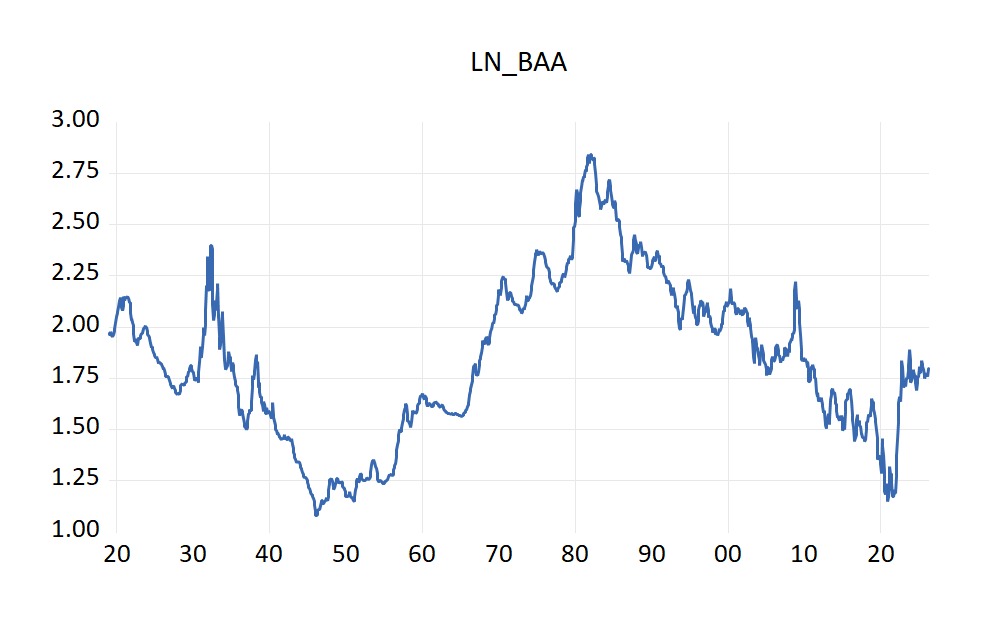
\includegraphics[width=0.8\textwidth]{log_open1.png}
\caption{对数收益率序列(LN\_BAA)时序图}
\label{fig:log_open1}
\end{figure}


\section{时间序列平稳性和非白噪声检验}

\subsection{时间序列平稳性检验}

由图~\ref{fig:log_open1}可观察出，序列LN\_BAA不是一个平稳的时间序列。下面通过单位根检验(ADF检验)严格检验序列LN\_BAA不是一个平稳的时间序列。

对序列LN\_BAA进行单位根检验（ADF检验），分别检验三种情形：无截距无趋势（左侧）、仅含截距（右下）、含截距+线性趋势（右上），结果如图~\ref{fig:adf_test1}所示。
\begin{figure}[H]
\centering
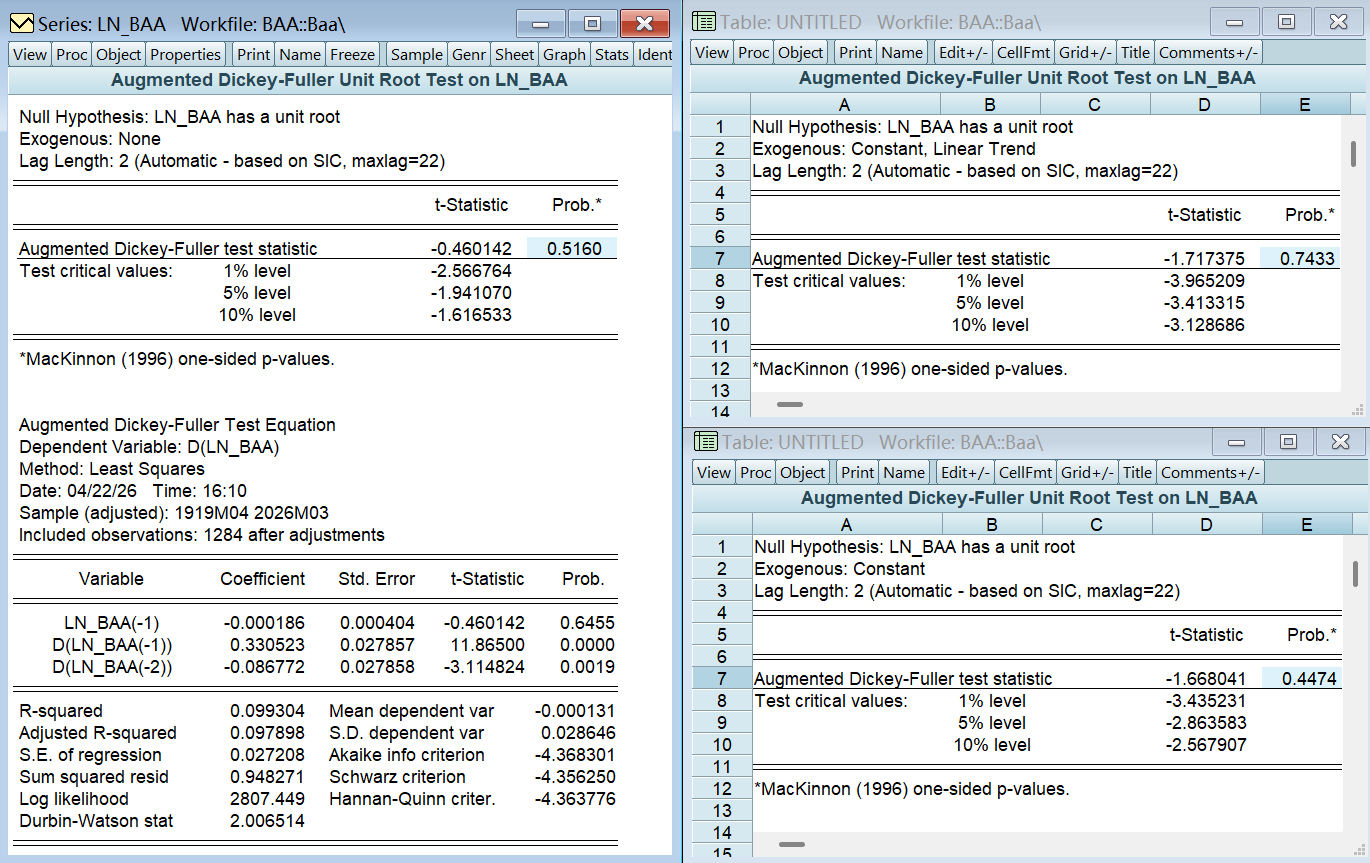
\includegraphics[width=0.8\textwidth]{adf_test1.png}
\caption{对数收益率序列(LN\_BAA)的单位根检验图}
\label{fig:adf_test1}
\end{figure}
由图~\ref{fig:adf_test1}可知，三种情形中，无截距无趋势模型的P值为 0.5160>0.05，仅含截距模型的P值为 0.4474>0.05，含截距+线性趋势模型的P值为 0.7433>0.05，在5\%显著性水平下均无法拒绝 “序列存在单位根” 的原假设。这说明，原序列LN\_BAA在三种检验设定下均存在单位根、不满足平稳性要求，因此，后续建模不能直接对原序列建立 ARMA 模型，需要先对序列进行差分处理，再对差分后的序列重新进行单位根检验，根据差分后的平稳性结果选择对应的模型形式。

对对数收益率序列(LN\_BAA)做一阶差分得
\begin{align}
\mathrm{DF}\_\mathrm{LN}\_\mathrm{BAA}=\mathrm{LN}\_\mathrm{BAA}_t-\mathrm{LN}\_\mathrm{BAA}_{t-1},
\end{align}
记为对数一阶差分收益率序列(DF\_LN\_BAA),其时序图如图~\ref{fig:dflog_open1}所示。
\begin{figure}[H]
\centering
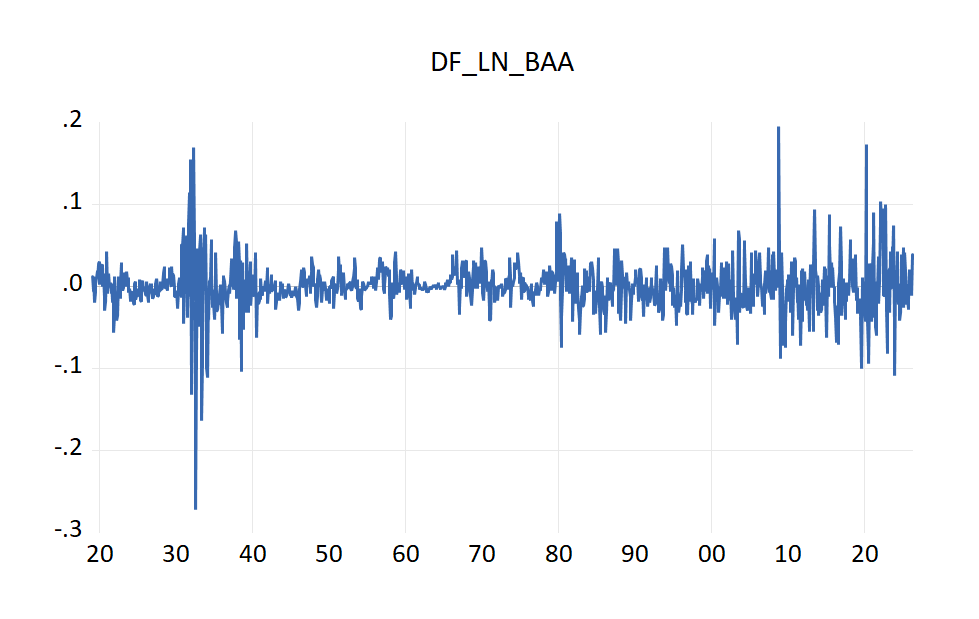
\includegraphics[width=0.8\textwidth]{dflog_open1.png}
\caption{对数一阶差分收益率序列(DF\_LN\_BAA)时序图}
\label{fig:dflog_open1}
\end{figure}
由图~\ref{fig:dflog_open1}可观察出，序列DF\_LN\_BAA是一个平稳的时间序列。下面通过单位根检验(ADF检验)严格证明序列DF\_LN\_BAA是一个平稳的时间序列。

对序列DF\_LN\_BAA进行单位根检验（ADF检验），分别检验三种情形：无截距无趋势（左）、仅含截距（中间）、含截距+线性趋势（右），结果如图~\ref{fig:adf_test2}所示。
\begin{figure}[H]
\centering
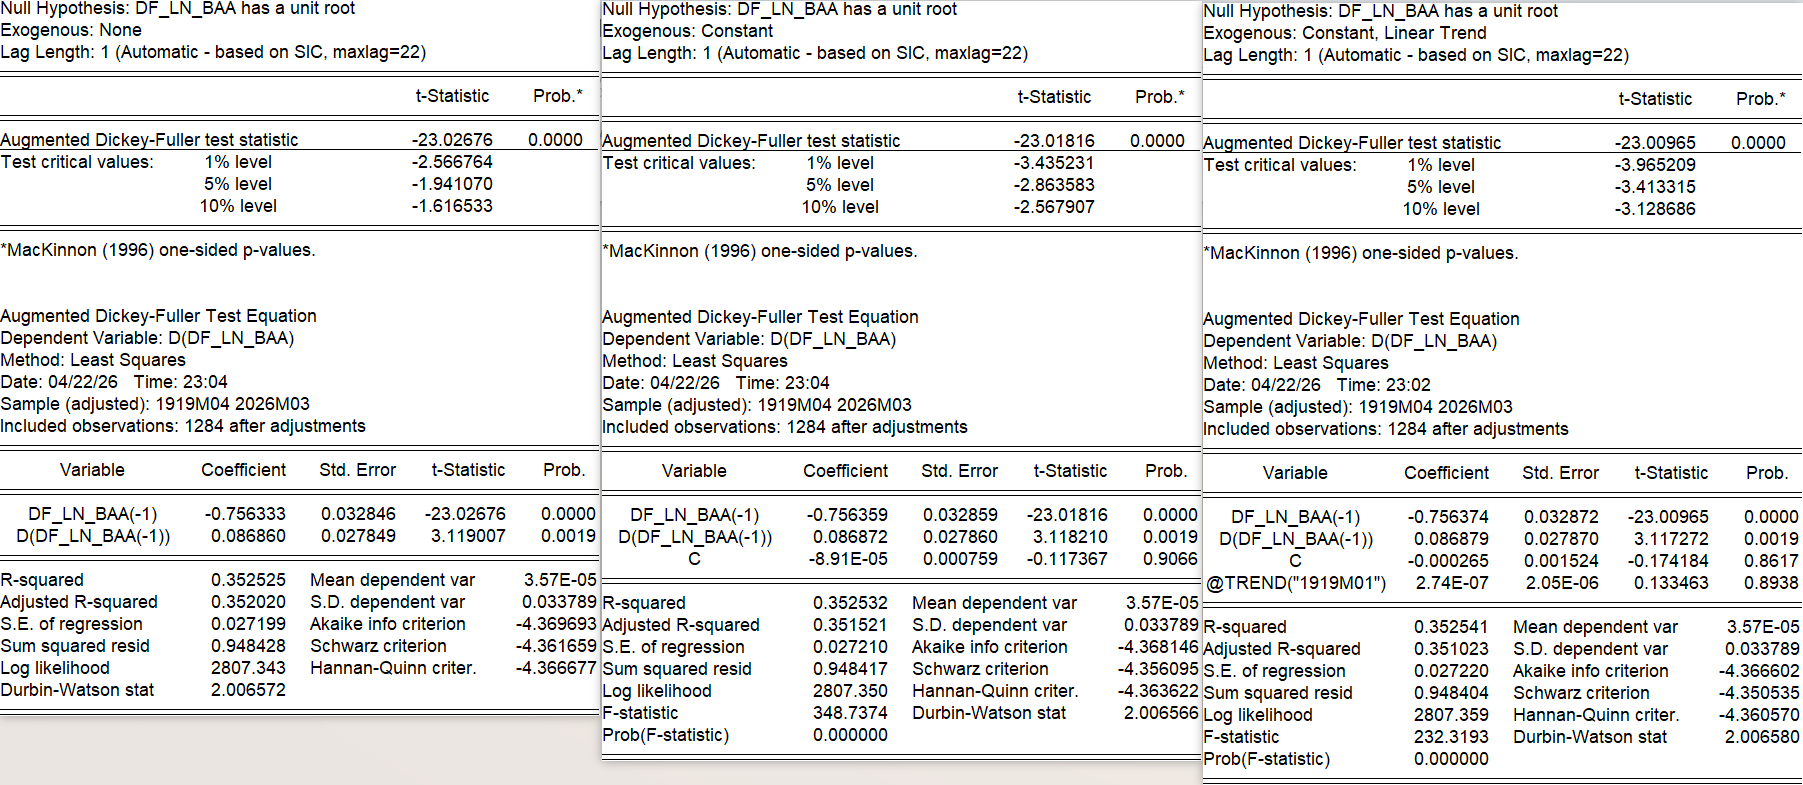
\includegraphics[width=0.8\textwidth]{adf_test2.png}
\caption{序列DF\_LN\_BAA的单位根检验图}
\label{fig:adf_test2}
\end{figure}
由图~\ref{fig:adf_test2}可知，三种情形的P值均为0.000<0.05，在5\%显著性水平下均拒绝 “序列存在单位根” 的原假设。这说明，序列DF\_LN\_BAA在三种检验设定下均不存在单位根、满足平稳性要求，即序列DF\_LN\_BAA为\textbf{平稳时间序列}。再整理图~\ref{fig:adf_test2}中三种情形的AIC/SC/HQ值如表~\ref{table:不同情形的信息准则对比}所示。
\begin{table}[H]
\centering
\caption{序列DF\_LN\_BAA单位根检验不同情形的信息准则对比}
\label{table:不同情形的信息准则对比}
\begin{tabular}{lccc}
\toprule[1.2pt] % 顶部粗线
检验设定 & AIC准则 & SC准则 & HQ准则 \\
\midrule[0.75pt] % 中间细线
None & $\mathbf{-4.369693}$ & $\mathbf{-4.361659}$ & $\mathbf{-4.366677}$ \\
Constant & -4.368146 & -4.356095 & -4.363622 \\
Constant,Linear Trend & -4.366602 & -4.350535 & -4.360570 \\
\bottomrule[1.2pt] % 底部粗线
\end{tabular}
\end{table}

根据AIC/SC/HQ准则，最终选择\textbf{无截距项、无线性趋势}$(\mathbf{None})$的情形，故可对序列DF\_LN\_BAA构建\textbf{无截距、无趋势的}$\mathbf{ARMA}$\textbf{模型}。

\subsection{非白噪声检验}

序列DF\_LN\_BAA的白噪声检验结果如图~\ref{fig:acf_pacf1}所示。
\begin{figure}[H]
\centering
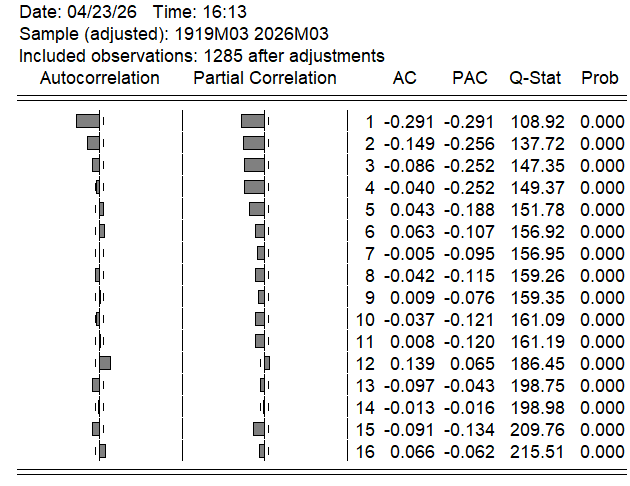
\includegraphics[width=0.8\textwidth]{acf_pacf1.png}
\caption{序列自相关(AC)、偏自相关(PAC)和白噪声检验图}
\label{fig:acf_pacf1}
\end{figure}
由图~\ref{fig:acf_pacf1}可知，序列DF\_LN\_BAA的白噪声检验结果：
\begin{itemize}
\item 序列的自相关系数（AC）在滞后 1 阶为 $-0.291$，显著为负且超出置信区间；后续多个滞后阶数（如 2、3、12、13、15 阶）的自相关系数也显著不为 0，说明序列存在显著的序列相关性，拒绝白噪声序列无自相关的基本假设。

\item 各滞后阶数对应的 Ljung-Box Q 统计量的 P 值均为 0.000，小于 0.01 的显著性水平，强烈拒绝序列为白噪声的原假设，进一步说明序列并非无信息的纯随机过程，存在显著的序列相关性，具备构建时间序列模型的信息基础。
\end{itemize}


\section{样本的自相关和偏自相关函数检验}

序列DF\_LN\_BAA的自相关与偏自相关图同样如图~\ref{fig:acf_pacf1}所示。结果分析如下：
\begin{itemize}
\item 自相关函数（ACF）特征：序列的自相关系数（AC）在滞后1阶为$-0.291$，显著不为0；随着滞后阶数增加，自相关系数未快速衰减并落入置信区间，部分高阶滞后（如第12、13、15阶）的自相关系数仍显著不为0，整体呈现\textbf{拖尾}特征。

\item 偏自相关函数（PACF）特征：序列的偏自相关系数（PAC）在滞后1阶为$-0.291$，显著不为0；后续部分高阶滞后（如第13阶）的偏自相关系数仍超出置信区间，未表现出快速截尾的特征，整体同样呈现\textbf{拖尾}特征，适合采用ARMA模型建模。
\end{itemize}


\section{模型识别、模型定阶与参数估计}

由图~\ref{fig:acf_pacf1}和之前的分析可知，序列DF\_LN\_BAA的ACF、PACF都呈\textbf{拖尾}特征，应选择ARMA模型进行建模。对序列DF\_LN\_BAA分别建立ARMA(1,1)、ARMA(1,2)、ARMA(1,3)、ARMA(2,1)、ARMA(2,2)、ARMA(2,3)、ARMA(3,1)、ARMA(3,2)、ARMA(3,3)模型，如图~\ref{fig:ARMA--1}、图~\ref{fig:ARMA--2}、图~\ref{fig:ARMA--3}所示。
\begin{figure}[H]
\centering
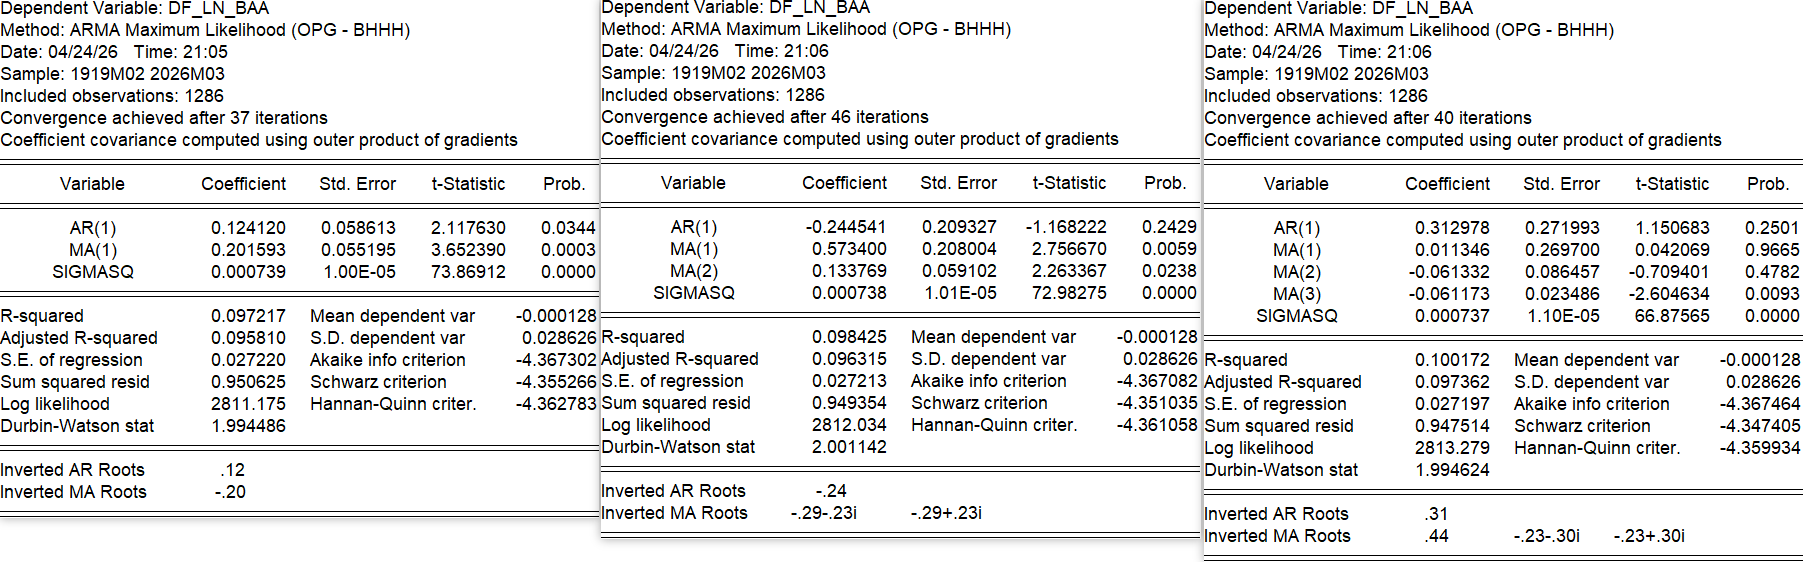
\includegraphics[width=0.8\textwidth]{ARMA--1.png}
\caption{ARMA(1,1)、ARMA(1,2)、ARMA(1,3)模型结果图}
\label{fig:ARMA--1}
\end{figure}
\begin{figure}[H]
\centering
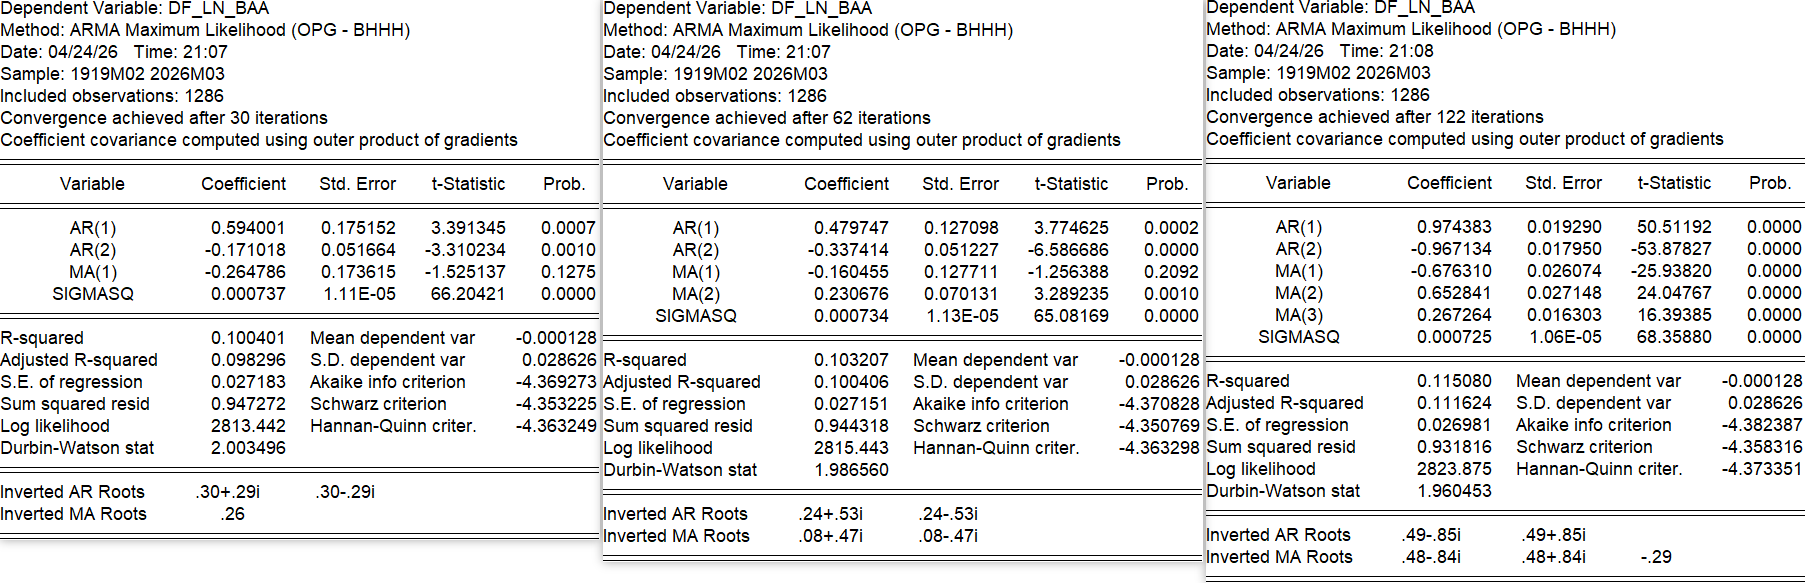
\includegraphics[width=0.8\textwidth]{ARMA--2.png}
\caption{ARMA(2,1)、ARMA(2,2)、ARMA(2,3)模型结果图}
\label{fig:ARMA--2}
\end{figure}
\begin{figure}[H]
\centering
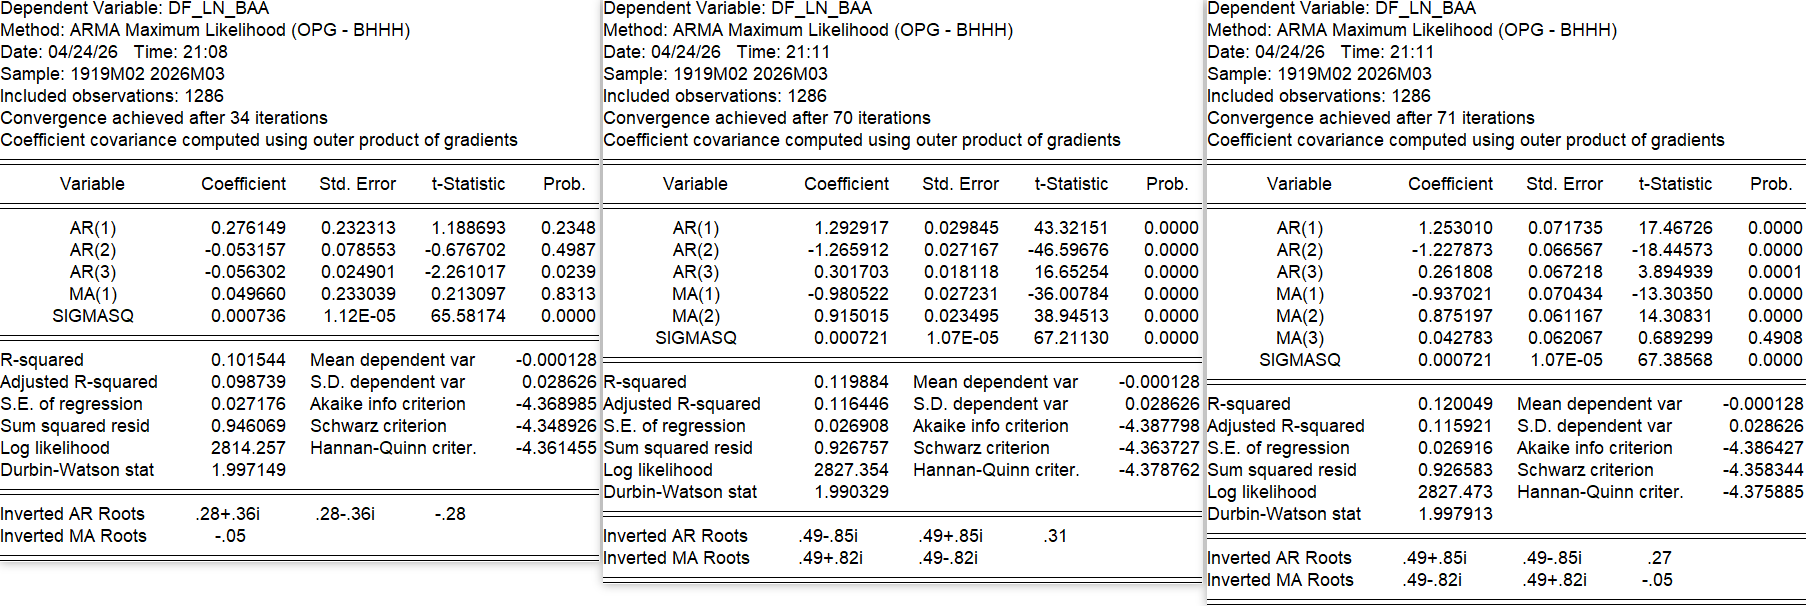
\includegraphics[width=0.8\textwidth]{ARMA--3.png}
\caption{ARMA(3,1)、ARMA(3,2)、ARMA(3,3)模型结果图}
\label{fig:ARMA--3}
\end{figure}
将图~\ref{fig:ARMA--1}、图~\ref{fig:ARMA--2}、图~\ref{fig:ARMA--3}中各个ARMA模型的系数显著性检验结果和AIC/SC/HQ值分别汇总到如下表~\ref{tab:arma_pvalue}和表~\ref{tab:arma_criteria}中。
\begin{table}[H]
\centering
\caption{ARMA模型系数显著性检验结果}
\label{tab:arma_pvalue}
% \footnotesize
\begin{tabular}{cccccccc}
\toprule[1.2pt] % 顶部粗线
模型  & AR(1) & AR(2) & AR(3) & MA(1) & MA(2) & MA(3) \\
\midrule[0.75pt] % 中间细线
ARMA(1,1)  & 0.0344 & - & - & 0.0003 & - & - \\
ARMA(1,2)  & 0.2429 & - & - & 0.0059 & 0.0238 & - \\
ARMA(1,3)  & 0.2501 & - & - & 0.9665 & 0.4782 & 0.0093 \\
ARMA(2,1)  & 0.0007 & 0.0010 & - & 0.1275 & - & - \\
ARMA(2,2)  & 0.0002 & 0.0000 & - & 0.2092 & 0.0010 & - \\
ARMA(2,3)  & 0.0000 & 0.0000 & - & 0.0000 & 0.0000 & 0.0000 \\
ARMA(3,1)  & 0.2348 & 0.4987 & 0.0239 & 0.8313  & - & - \\
ARMA(3,2) & 0.0000 & 0.0000 & 0.0000 & 0.0000 & 0.0000 & - \\
ARMA(3,3) & 0.0000 & 0.0000 & 0.0001 & 0.0000 & 0.0000 & 0.4908 \\
\bottomrule[1.2pt] % 底部粗线
\end{tabular}
\end{table}

\begin{table}[H]
\centering
\caption{ARMA模型信息准则对比结果}
\label{tab:arma_criteria}
% \footnotesize
\begin{tabular}{cccc}
\toprule[1.2pt]
模型 & AIC & SC & HQ \\
\midrule[0.75pt]
ARMA(1,1) & -4.3673 & -4.3553 & -4.3628 \\
ARMA(1,2) & -4.3671 & -4.3510 & -4.3611 \\
ARMA(1,3) & -4.3675 & -4.3474 & -4.3599 \\
ARMA(2,1) & -4.3693 & -4.3532 & -4.3632 \\
ARMA(2,2) & -4.3708 & -4.3508 & -4.3633 \\
ARMA(2,3) & -4.3824 & -4.3583 & -4.3734 \\
ARMA(3,1) & -4.3690 & -4.3489 & -4.3615 \\
ARMA(3,2) & $\mathbf{-4.3878}$ & $\mathbf{-4.3637}$ & $\mathbf{-4.3788}$ \\
ARMA(3,3) & -4.3864 & -4.3583 & -4.3759 \\
\bottomrule[1.2pt]
\end{tabular}
\end{table}
由表~\ref{tab:arma_pvalue}和表~\ref{tab:arma_criteria}可知：
\begin{itemize}
\item 从系数显著性来看，ARMA(1,1)、ARMA(2,3)、ARMA(3,2) 模型中所有自回归项(AR)与移动平均项(MA)的系数均高度显著，说明各项滞后结构均具备明确的统计意义。而其余模型至少有一个系数不显著。

\item 从信息准则角度，ARMA (3,2) 模型的 AIC、SC 与 HQ 信息准则值均为全部模型中最小，表明该模型在序列拟合效果与模型复杂程度之间达到了最优平衡。
\end{itemize}
综合以上判断，最终选择 $\mathbf{ARMA}(\mathbf{3},\mathbf{2})$\textbf{模型}进行后续建模与分析。其余模型或存在部分滞后项系数不显著的问题，或在信息准则上表现更差。


\section{模型适应性检验}

对 ARMA (3,2) 模型的残差序列进行 Ljung-Box Q 检验，以验证残差是否满足白噪声假设，检验结果如图~\ref{fig:acf_pacf2}所示。
\begin{figure}[H]
\centering
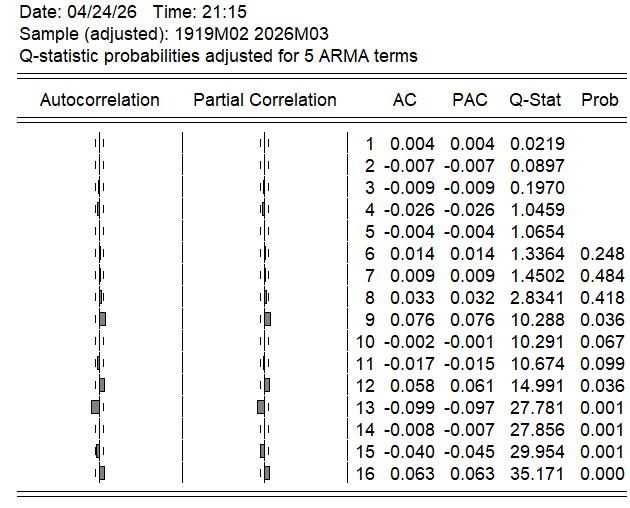
\includegraphics[width=0.8\textwidth]{acf_pacf2.png}
\caption{ARMA(3,2)模型残差序列的ACF与PACF相关图}
\label{fig:acf_pacf2}
\end{figure}
由图~\ref{fig:acf_pacf2}可知：
\begin{itemize}
\item ARMA(3,2)模型残差在核心低阶滞后（1-8 阶）均无显著自相关：残差的自相关系数（AC）与偏自相关系数（PAC）均未超出置信区间，对应的 Q 统计量 P 值均大于 0.05 的显著性水平，无法拒绝 “残差为白噪声” 的原假设，说明 ARMA (3,2) 模型已充分提取了序列的主要自相关信息，对数据的短期动态特征拟合效果良好。

\item 对于少数高阶滞后（如第 9、12 阶及以后）出现的 Q 统计量显著情况，结合样本量较大（1286 个观测值）的背景来看，这类高阶微弱的统计显著性，更多是由数据中的随机噪声或非系统性波动导致，并未形成持续的序列相关性，对模型的整体有效性与参数估计的一致性的影响较小。
\end{itemize}
综上可知，ARMA (3,2) 模型的残差基本符合白噪声假设，说明ARMA (3,2)模型\textbf{已有效捕捉序列的核心动态特征}，满足时间序列建模的基本要求。


\section{确定ARMA模型}

根据之前的分析可知，ARMA(3,2)模型的AIC/SC/HQ信息准则值均为全部ARMA模型中最小，所有的自回归项与移动平均项系数的P值均高度显著，而且ARMA(3,2)模型的残差基本符合白噪声假设，故可确定序列DF\_LN\_BAA的ARMA模型为$\mathbf{ARMA(}\mathbf{3},\mathbf{2)}$\textbf{模型}。序列DF\_LN\_BAA的ARMA(3,2)模型估计结果如图~\ref{fig:BAAARMA32}所示。
\begin{figure}[H]
\centering
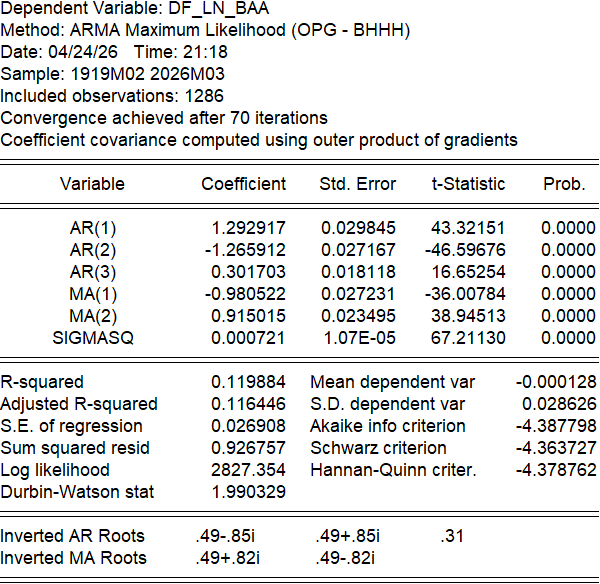
\includegraphics[width=0.8\textwidth]{BAAARMA32.png}
\caption{序列DF\_LN\_BAA的ARMA(3,2)模型估计结果图}
\label{fig:BAAARMA32}
\end{figure}
序列DF\_LN\_BAA的ARMA(3,2)模型的形式为
\begin{gather}\label{eq:iowhjfwjf903eg6ersgdrsgsggggggggggg}
\begin{aligned}
\text{DF\_LN\_BAA}_t &= \phi_1 \, \text{DF\_LN\_BAA}_{t-1} + \phi_2 \, \text{DF\_LN\_BAA}_{t-2}  
\\
&\quad + \phi_3 \, \text{DF\_LN\_BAA}_{t-3} + \theta_1 \, \varepsilon_{t-1} + \theta_2 \, \varepsilon_{t-2} + \varepsilon_t
\end{aligned}
\end{gather}
其中，$\phi_1, \phi_2, \phi_3$为自回归(AR)系数；$\theta_1, \theta_2$为移动平均(MA)系数；$\varepsilon_t$为残差项。
将图~\ref{fig:BAAARMA32}中的模型估计结果代入\eqref{eq:iowhjfwjf903eg6ersgdrsgsggggggggggg}式得
\begin{gather}\label{eq::02jr20j390irjkw0edzgdfzgggggfdss}
\begin{aligned}
\text{DF\_LN\_BAA}_t&= 1.292917 \, \text{DF\_LN\_BAA}_{t-1} 
- 1.265912 \, \text{DF\_LN\_BAA}_{t-2}    
\\
&\quad + 0.301703 \, \text{DF\_LN\_BAA}_{t-3}
- 0.980522 \, \varepsilon_{t-1} 
\\
&\quad + 0.915015 \, \varepsilon_{t-2} + \varepsilon_t,
\end{aligned}
\end{gather}
其中，残差项$\varepsilon_t \sim N(0, \sigma^2)$，方差估计值为 $\sigma^2 = 0.000721$。

由\eqref
{eq::02jr20j390irjkw0edzgdfzgggggfdss}式可知，ARMA(3,2)模型的自回归系数 $\phi_1$、$\phi_2$、$\phi_3$与移动平均系数 $\theta_1$、$\theta_2$ 均在 1\% 的显著性水平下显著，说明序列存在显著的三阶自相关特征与二阶滞后冲击效应，当期收益率受自身历史值与过去随机冲击的影响具有显著的动态相关性。

\section{异方差检验}

\subsection{初步判断}

序列DF\_LN\_BAA的直方图与描述性统计如图~\ref{fig:df_ln_baa_data}所示。
\begin{figure}[H]
\centering
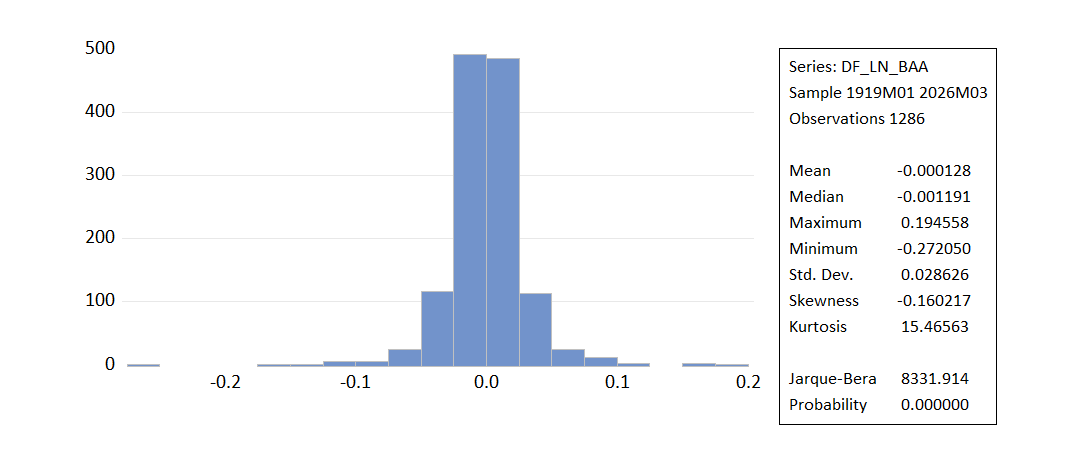
\includegraphics[width=0.8\textwidth]{df_ln_baa_data.png}
\caption{序列DF\_LN\_BAA的直方图与描述性统计}
\label{fig:df_ln_baa_data}
\end{figure}

由图~\ref{fig:df_ln_baa_data}可知，序列DF\_LN\_BAA的均值与中位数均接近 0，整体分布近似对称(偏度为 - 0.1602)；但峰度高达 15.4656，远高于正态分布的峰度值 3，说明序列分布呈现显著的\textbf{尖峰厚尾}特征，即分布的中心峰值更陡峭，且尾部概率显著大于正态分布，存在较多极端值。同时，Jarque-Bera 正态性检验的统计量为 8331.91，对应的 P 值为 0.0000，强烈拒绝序列服从正态分布的原假设，进一步印证了序列的\textbf{非正态性}与\textbf{尖峰厚尾}特征。

序列DF\_LN\_BAA的ARMA(3,2)模型的实际值、拟合值与残差时序图，如图~\ref{fig:df_ln_baa_data_figure}所示。
\begin{figure}[H]
\centering
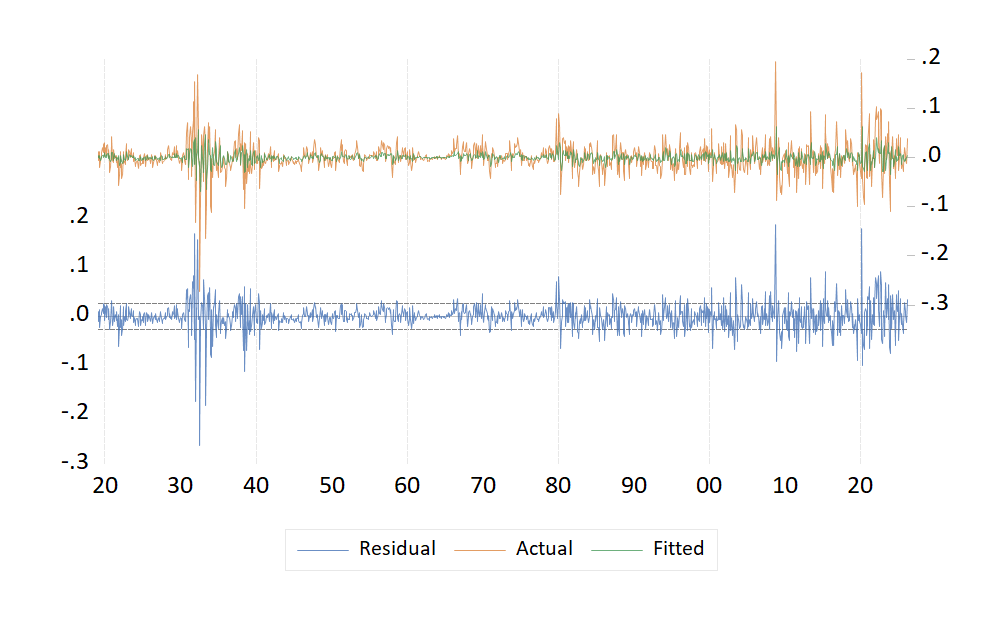
\includegraphics[width=0.8\textwidth]{df_ln_baa_data_figure.png}
\caption{ARMA(3,2)模型的实际值、拟合值与残差时序图}
\label{fig:df_ln_baa_data_figure}
\end{figure}
根据图~\ref{fig:df_ln_baa_data_figure}可以直观地观察到，模型残差的波动并非恒定不变，而是呈现出明显的\textbf{波动聚集效应}，即在部分时段，残差的波动幅度显著增大，大波动往往连续出现；而在其他时段，残差则表现为持续的低波动状态。这说明序列的方差存在条件异方差性，普通 ARMA 模型的同方差假设无法刻画这种波动聚集特征，因此需要引入 ARCH/GARCH 模型，对序列的均值方程与方差方程进行联合建模，以同时捕捉序列的均值回归与波动聚集特征。

下面采用ARCH-LM检验与残差平方的Ljung-Box Q检验两种互补方法严格验证 ARMA(3,2)模型残差存在条件异方差性。

\subsection{严格检验}

\subsubsection{ARCH-LM检验}

对序列DF\_LN\_BAA的ARMA(3,2)模型的残差做滞后1阶的ARCH效应检验，结果如图~\ref{fig:ARMA32-1}所示。
\begin{figure}[H]
\centering
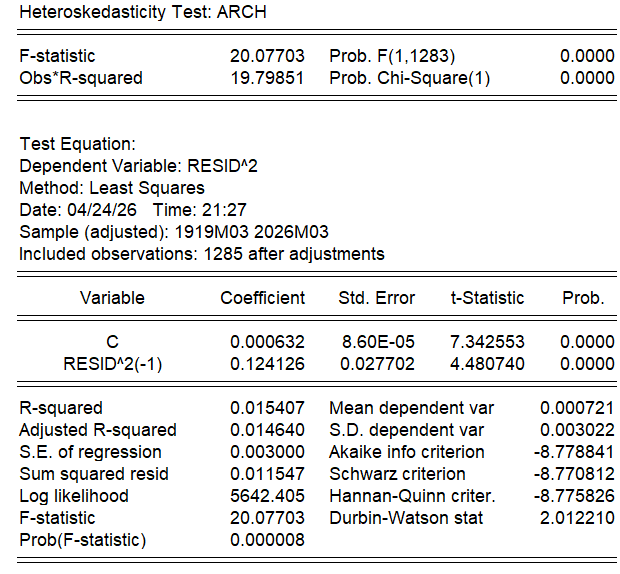
\includegraphics[width=0.8\textwidth]{ARMA32-1.png}
\caption{ARMA(3,2)模型残差的 ARCH 效应检验结果图}
\label{fig:ARMA32-1}
\end{figure}
根据图~\ref{fig:ARMA32-1}可知，F 统计量与 Obs*R-squared（LM 统计量）对应的 P 值均为 0.0000，远小于 1\% 的显著性水平，强烈拒绝 “残差不存在 ARCH 效应” 的原假设，初步判断残差存在条件异方差。

\subsubsection{Ljung-Box Q检验}

再对序列DF\_LN\_BAA的ARMA(3,2)模型的残差平方做Ljung-Box Q 检验，结果如图~\ref{fig:ARMA32CRS}所示。
\begin{figure}[H]
\centering
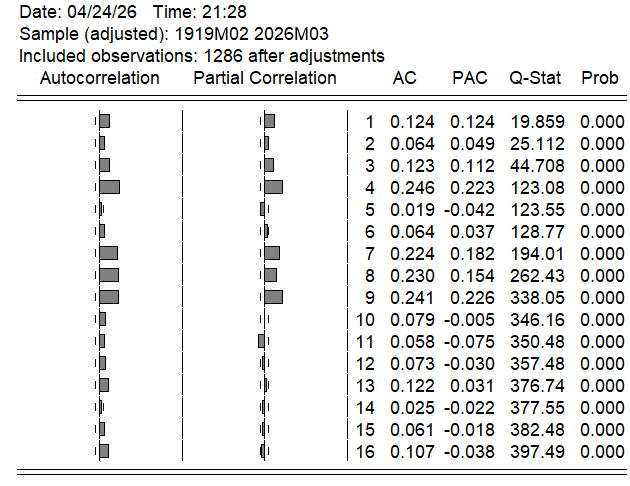
\includegraphics[width=0.8\textwidth]{ARMA32CRS.png}
\caption{ARMA(3,2)模型残差平方序列的ACF与PACF相关图}
\label{fig:ARMA32CRS}
\end{figure}
图~\ref{fig:ARMA32CRS}的检验结果显示：
\begin{itemize}
\item 残差平方序列的自相关函数（ACF）在滞后 1、4、7-9 阶等多个阶数均显著超出置信区间，且未呈现快速衰减的特征；偏自相关函数（PACF）同样在多个高阶滞后显著不为 0。这说明，残差的方差存在显著且持续的自相关，即序列波动呈现出明显的\textbf{聚集性}，ARCH 效应不仅存在，且具有持续性。

\item 滞后 1 至 16 阶的 Q 统计量对应的 P 值均为 0.0000<0.01，强烈拒绝 “残差平方序列无自相关” 的原假设，进一步验证了残差平方序列的序列相关性，序列波动呈现出明显的\textbf{聚集性}特征。
\end{itemize}
综上所述，ARCH-LM检验与残差平方的Ljung-Box Q检验互相印证，共同证明了 ARMA (3,2) 模型的残差存在显著且持续的条件异方差（ARCH 效应）。这说明普通 ARMA 模型仅刻画了序列的均值动态特征，未能捕捉其波动层面的聚集性规律，同方差假设已不成立。为修正异方差带来的估计偏差，同时全面刻画序列的均值回归与波动聚集双重特征，后续将重新构建 ARCH/GARCH 模型，对序列DF\_LN\_BAA的均值方程与方差方程进行联合建模。


\section{建立ARCH模型}

经过之前的ARCH效应检验，发现ARMA模型残差存在显著的条件异方差，违背了经典时间序列模型的同方差假设。为同时刻画序列的均值动态与波动聚集性，现在构建GARCH族模型对序列DF\_LN\_BAA进行建模。

下面分别建立GARCH、TARCH、EGARCH三种模型，由图~\ref{fig:df_ln_baa_data}知，序列DF\_LN\_BAA呈现非正态性与\textbf{尖峰厚尾}特征，即序列更符合Student's t分布的特征，因此，这三种模型都\textbf{采用}$\mathbf{Student}' \mathbf{s}\,\,\mathbf{t}$\textbf{分布}进行建模。

由于金融序列的波动聚集性通常可由低阶 GARCH 模型充分捕捉，高阶模型易引入冗余参数，导致过拟合或估计不稳定。同时遵循模型简约性原则，在拟合效果相近的情况下，选择低阶模型更优，为避免不必要的复杂度，本文这三种模型的方差方程均采用金融时间序列的通用基准设定，即$\mathbf{ARCH}$、$\mathbf{GARCH}$\textbf{的阶数都固定为}$\mathbf{1}$\textbf{阶}。

再根据联合估计下的系数显著性对均值方程进行精简，\textbf{剔除不显著项}，保证联合估计的有效性，最终确定各个模型的阶数。

\subsection{建立ARMA-GARCH模型}

对序列DF\_LN\_BAA建立ARMA(3,2)-GARCH(1,1)模型，如图~\ref{fig:GARMA11}所示。
\begin{figure}[H]
\centering
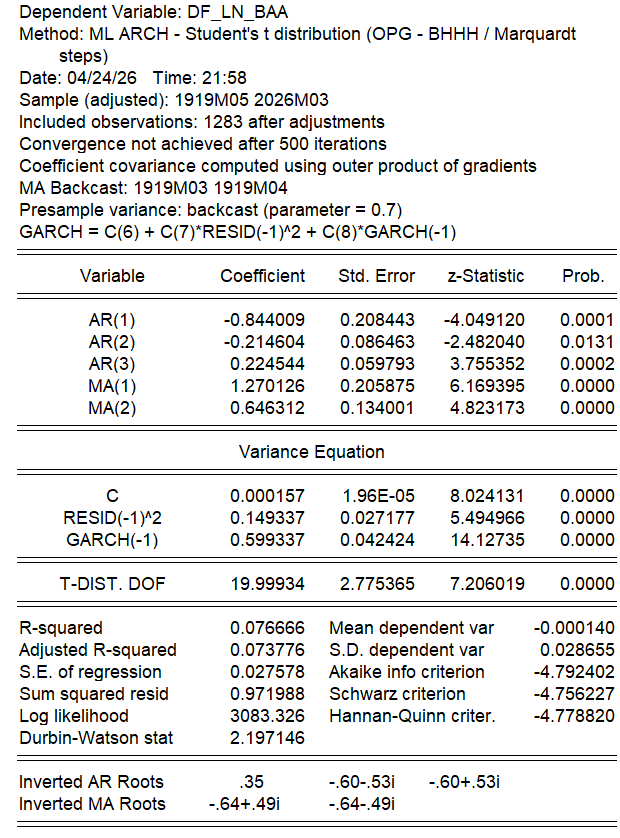
\includegraphics[width=0.8\textwidth]{GARMA11.png}
\caption{ARMA(3,2)-GARCH(1,1)模型估计结果图}
\label{fig:GARMA11}
\end{figure}
图~\ref{fig:GARMA11}显示，ARMA (3,2)-GARCH (1,1) 的均值方程与方差方程的各参数系数均在 5\% 的显著性水平下显著，模型参数估计有效。

\subsection{建立ARMA-EGARCH模型}

对序列DF\_LN\_BAA建立ARMA(3,2)-EGARCH(1,1)模型，如图~\ref{fig:EARMA11}所示。
\begin{figure}[H]
\centering
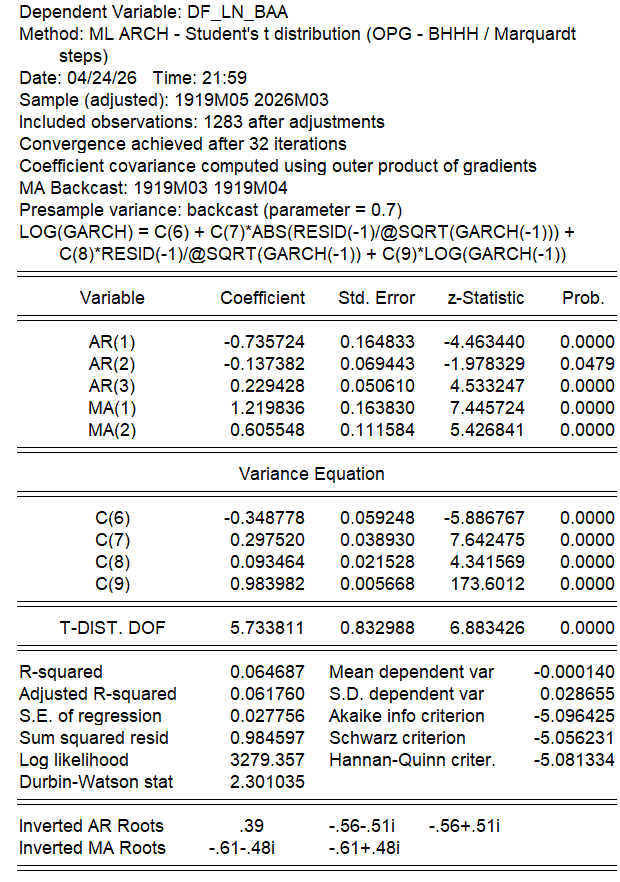
\includegraphics[width=0.8\textwidth]{EARMA11.png}
\caption{ARMA(3,2)-EGARCH(1,1)模型估计结果图}
\label{fig:EARMA11}
\end{figure}
图~\ref{fig:EARMA11}显示：
\begin{itemize}
\item ARMA (3,2)-EGARCH (1,1) 的均值方程与方差方程的各参数系数均在 5\% 的显著性水平下显著，模型参数估计有效。

\item 方差方程中ARCH项、非对称项及 GARCH项系数均显著，且非对称项系数C(8)=0.093464显著为正，说明\textbf{序列存在反向杠杆效应}，即同等强度的正向冲击对波动的影响大于负向冲击。
\end{itemize}


\subsection{建立ARMA-TARCH模型}

对序列DF\_LN\_BAA建立ARMA(3,2)-TARCH(1,1)模型，如图~\ref{fig:TARCH11111}所示。
\begin{figure}[H]
\centering
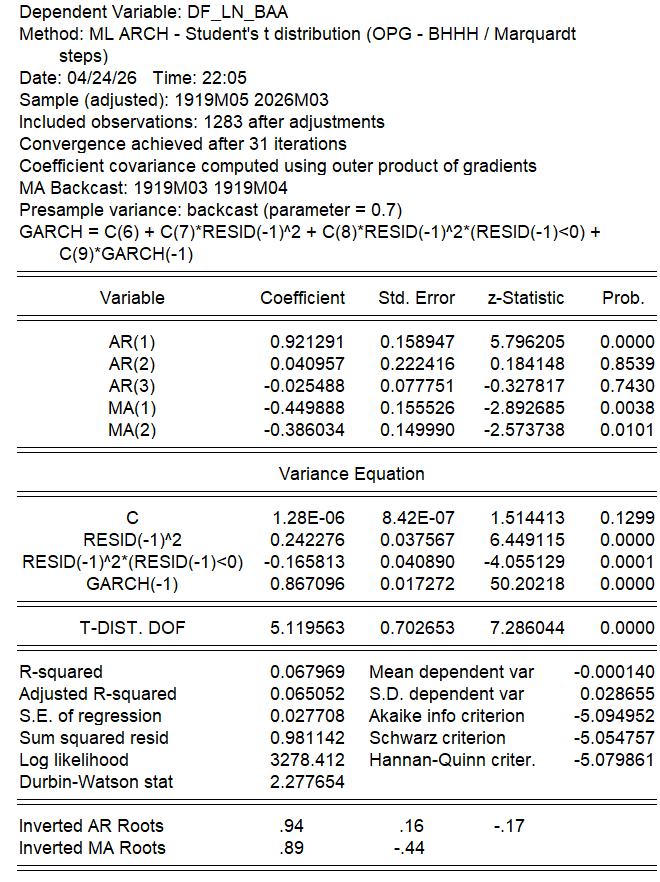
\includegraphics[width=0.8\textwidth]{TARCH11.png}
\caption{ARMA(3,2)-TARCH(1,1)模型估计结果图}
\label{fig:TARCH11111}
\end{figure}
由图~\ref{fig:TARCH11111}可知，ARMA(3,2)-TARCH(1,1)模型的自回归项AR(2)、AR(3)的系数P值分别为0.8539、0.7430>0.05，在5\%的显著性水平下不显著。因此，同时剔除不显著的AR(2)、AR(3)项，得到ARMA(1,2)-TARCH(1,1)模型，如图~\ref{fig:12TARCH11}所示。
\begin{figure}[H]
\centering
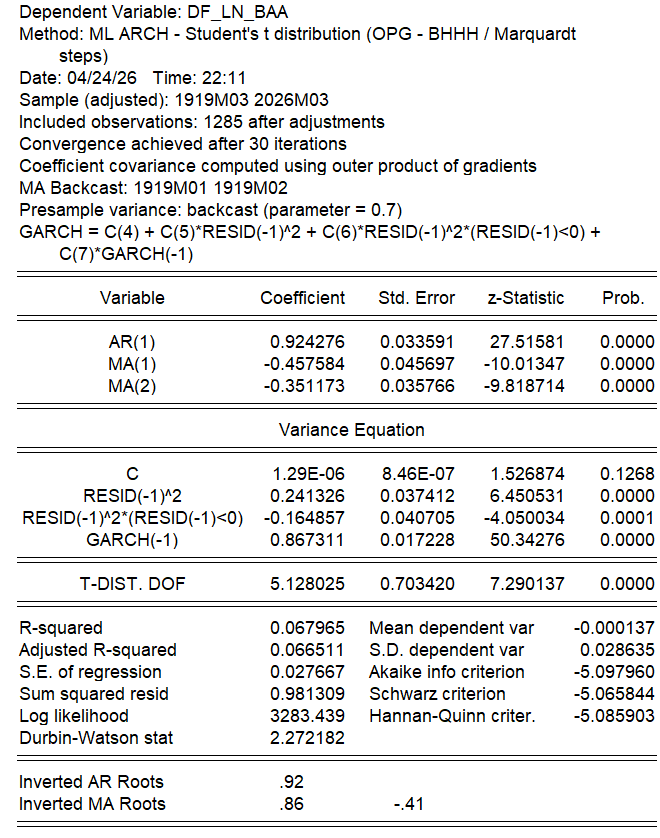
\includegraphics[width=0.8\textwidth]{12TARCH11.png}
\caption{ARMA(1,2)-TARCH(1,1)模型估计结果图}
\label{fig:12TARCH11}
\end{figure}
由图~\ref{fig:12TARCH11}可知，方差方程常数项\( \omega=1.29\times10^{-6} \)的p值为0.1268，在常规显著性水平下不显著，但\textbf{该不显著性不影响模型的有效性}。这是因为：
\begin{itemize}
\item 常数项数值极小、近似为0；

\item GARCH类模型的核心关注对象为ARCH、GARCH及非对称项的显著性，本模型中上述核心变量均在5\%水平下高度显著，已成功捕捉序列的波动聚类、持续性与非对称特征；

\item 由于ARCH与GARCH项系数之和大于1，波动过程存在强持续性，序列不存在稳定的长期无条件方差，常数项所代表的无条件方差基准水平的经济意义被弱化，其统计不显著具有理论合理性。
\end{itemize}

因此，本文保留原模型设定。图~\ref{fig:12TARCH11}还显示：
\begin{itemize}
\item 均值方程中，AR(1)、MA(1)、MA(2)系数均在 5\% 的显著性水平下高度显著，说明序列DF\_LN\_BAA存在显著的自相关与移动平均效应，前期收益率与滞后冲击对当期值具有显著影响；

\item 方差方程中 ARCH 项系数显著为正，说明\textbf{序列存在显著的波动聚类效应}；GARCH 项系数显著为正，且 ARCH 与 GARCH 项系数之和约为 1.108，说明\textbf{波动具有极强的持续性}；

\item 杠杆项系数显著为负，正向冲击对波动的直接影响为 0.2413，负向冲击对波动的总影响为0.2413−0.1648=0.0765，负向冲击带来的波动显著小于正向冲击，说明\textbf{序列存在反杠杆效应}，与传统杠杆效应相反。
\end{itemize}



\subsection{选取最优GARCH模型}

将图~\ref{fig:GARMA11}、图~\ref{fig:EARMA11}、图~\ref{fig:12TARCH11}中各个GARCH模型的AIC/SC/HQ信息准则值汇总到如下表~\ref{tab:garch_criteria}中。
\begin{table}[H]
\centering
\caption{GARCH族模型信息准则对比}
\label{tab:garch_criteria}
\begin{tabular}{cccc}
\toprule[1.2pt] % 顶部粗线
模型形式 & AIC & SC & HQ \\
\midrule[0.75pt] % 中间细线
ARMA(3,2)-GARCH(1,1) & -4.792402 & -4.756227 & -4.778820 \\
ARMA(3,2)-EGARCH(1,1) & -5.096425 & -5.056231 & -5.081334 \\
ARMA(1,2)-TARCH(1,1) & -5.097960 & -5.065844 & -5.085903 \\
\bottomrule[1.2pt] % 底部粗线
\end{tabular}
\end{table}
根据表~\ref{tab:garch_criteria}可知，$\mathbf{ARMA}(\mathbf{1},\mathbf{2})-\mathbf{TARCH}(\mathbf{1},\mathbf{1})$\textbf{模型}为最优模型，具体结果如图~\ref{fig:12TARCH11}所示。
由图~\ref{fig:12TARCH11}可知，ARMA(1,2)-TARCH(1,1)模型的均值方程为
\begin{gather}\label{eq:TARCH11-ARMA}
\begin{aligned}
\mathrm{DF}\_\mathrm{LN}\_\mathrm{BAA}_t &= \phi _1\,\mathrm{DF}\_\mathrm{LN}\_\mathrm{BAA}_{t-1}+\theta _1\,\varepsilon _{t-1}+\theta _2\,\varepsilon _{t-2}+\varepsilon _t
\\
&= 0.924276\,\mathrm{DF}\_\mathrm{LN}\_\mathrm{BAA}_{t-1}
\\
&\quad - 0.457584\,\varepsilon _{t-1} - 0.351173\,\varepsilon _{t-2}+\varepsilon _t,
\end{aligned}
\end{gather}
其中，\( \phi_1 = 0.924276 \) 为一阶自回归项系数，\( \theta_1 = -0.457584 \)、\( \theta_2 = -0.351173 \) 分别为一阶、二阶移动平均项系数，\( \varepsilon_t \sim t(\nu) \) 为服从\(\mathrm{Student}' \mathrm{s}\,\,\mathrm{t} \)分布的误差项，自由度\( \nu = 5.128025 \)。由\eqref{eq:TARCH11-ARMA}式可知
\begin{itemize}
\item 自回归系数\( \phi_1 = 0.924276 \)高度显著为正，说明序列\(\mathrm{DF}\_\mathrm{LN}\_\mathrm{BAA}\)存在显著的一阶正向自相关，当期值受前一期取值的同向影响较强，序列具有较强的短期持续性；

\item 移动平均系数\( \theta_1 = -0.457584 \)、\( \theta_2 = -0.351173 \)均高度显著为负，说明序列存在显著的滞后冲击修正效应，前两期的随机冲击会对当期值产生反向影响。
\end{itemize}

由图~\ref{fig:12TARCH11}可知，ARMA(1,2)-TARCH(1,1)模型的方差方程为
\begin{gather}\label{eq:TARCH11-VAR}
\begin{aligned}
\sigma_t^2 &= \omega + \alpha \varepsilon_{t-1}^2 + \gamma \varepsilon_{t-1}^2 \cdot I(\varepsilon_{t-1}<0) + \beta \sigma_{t-1}^2
\\
&= 1.29\times10^{-6} + 0.241326\,\varepsilon_{t-1}^2 
\\
&\quad - 0.164857\,\varepsilon_{t-1}^2 \cdot I(\varepsilon_{t-1}<0) + 0.867311\,\sigma_{t-1}^2,
\end{aligned}
\end{gather}
其中，\( \omega = 1.29\times10^{-6} \) 为方差方程常数项，\( \alpha = 0.241326 \) 为ARCH项系数，\( \gamma = -0.164857 \) 为非对称（杠杆）效应系数，\( \beta = 0.867311 \) 为GARCH项系数，\( I(\cdot) \) 为指示函数（当\( \varepsilon_{t-1}<0 \)时取1，否则取0），\( \sigma_t^2 \) 为条件方差。由\eqref{eq:TARCH11-VAR}式可知
\begin{itemize}
\item GARCH项系数\( \beta=0.867311 \)高度显著为正，且与ARCH项系数$\alpha$之和约为\( 0.241326+0.867311=1.1086>1 \)，说明序列的条件方差具有极强的\textbf{波动持续性}，外部冲击对波动的影响衰减速度极慢，市场波动存在显著的长记忆性；

\item ARCH项系数\( \alpha=0.241326 \)高度显著为正，说明序列存在显著的\textbf{波动聚类效应}；

\item 非对称项系数\( \gamma=-0.164857 \)高度显著为负，同等强度的正向冲击对波动的影响为\( 0.241326 \)，负向冲击对波动的总影响为\( 0.241326-0.164857=0.076469 \)，即正向冲击带来的波动显著大于负向冲击，说明序列存在\textbf{反杠杆效应}，与传统金融资产“负向冲击加剧波动”的杠杆效应相反。
\end{itemize}


\section{残差的白噪声检验}

\subsection{ARCH-LM检验}

由于原数据(BAA)是月度频率，滞后4阶刚好对应 “季度波动周期”，能覆盖月度金融数据中最常见的低阶异方差效应。因此，为验证 ARMA (1,2)-TARCH (1,1) 模型是否已充分捕捉序列DF\_LN\_BAA的条件异方差，只对标准化残差进行\textbf{滞后4阶}的 ARCH-LM 检验，结果如图~\ref{fig:EARCHLM1}所示。
\begin{figure}[H]
\centering
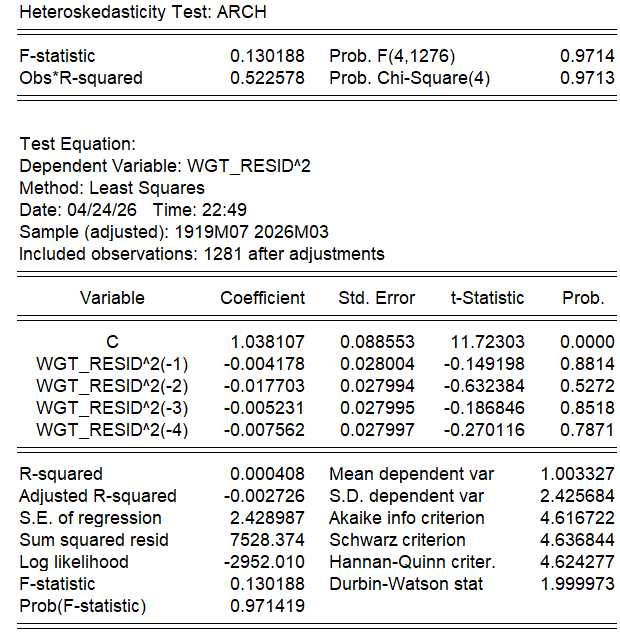
\includegraphics[width=0.8\textwidth]{EARCHLM1.png}
\caption{ARMA (1,2)-TARCH (1,1) 模型滞后 4 阶的 ARCH-LM 检验图}
\label{fig:EARCHLM1}
\end{figure}
图~\ref{fig:EARCHLM1}显示，F 统计量对应的 P 值为 0.9714，Obs*R-squared 对应的卡方检验 P 值为 0.9713，均显著大于 0.05 的显著性水平，无法拒绝 “残差不存在条件异方差” 的原假设。这表明ARMA(1,2)-TARCH(1,1)模型\textbf{已充分捕捉序列的波动聚集性与条件异方差特征}，\textbf{不存在剩余}$\mathbf{ARCH}$\textbf{效应}，模型设定合理有效。

\subsection{残差的白噪声检验}

对ARMA(1,2)-TARCH(1,1)模型的标准化残差进行 Ljung-Box Q 检验，结果如图~\ref{fig:EARCHLMQ}所示。
\begin{figure}[H]
\centering
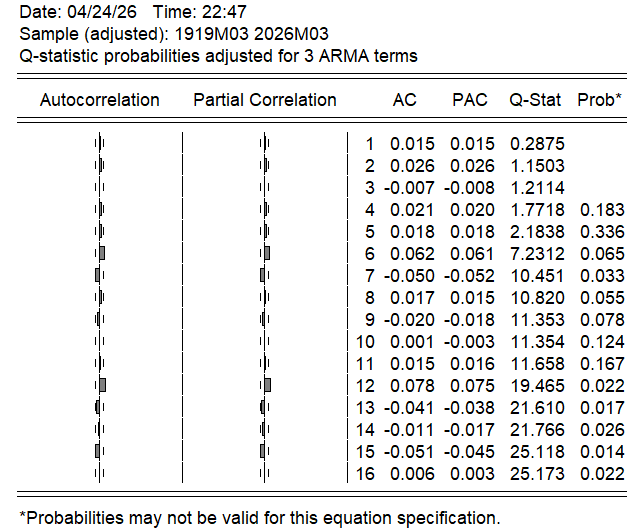
\includegraphics[width=0.8\textwidth]{EARCHLMQ.png}
\caption{ARMA (1,2)-TARCH (1,1) 模型残差序列的 ACF 与 PACF 相关图}
\label{fig:EARCHLMQ}
\end{figure}
图~\ref{fig:EARCHLMQ}中出现 “Probabilities may not be valid for this equation specification” 提示，这是 GARCH 类模型残差检验的常规现象。传统 Ljung-Box Q 检验要求残差满足独立同分布与同方差假设，而 TARCH 模型刻画的是时变条件异方差，违背了检验的原始假设，因此软件提示P值的严格有效性受限。

但从图~\ref{fig:EARCHLMQ}中的检验结果看，滞后 1-5 阶的 Q 统计量 P 值均大于 0.05 的显著性水平，无法拒绝 “残差无自相关” 的原假设，说明序列的低阶自相关已被模型充分捕捉。尽管滞后6阶及以后部分统计量显著，但月度数据高阶波动效应微弱，且大样本下少量高阶显著不影响模型整体有效性。综合来看，$\mathbf{ARMA(}\mathbf{1},\mathbf{2)}-\mathbf{TARCH(}\mathbf{1},\mathbf{1)}$\textbf{模型残差近似为白噪声}，\textbf{均值方程设定合理，已充分吸收序列的自相关特征}。


\end{document}